% overview
% Encoding
% Crossover \& Mutation
% Fitness function:
% - CF
% - LCS
% - Deepcoder
% Neighborhood search:
% - parametric neighborhood search
% - BFS
% - DFS
% In implementation/result section, talk about training data generation

%We will start with a high level overview of \scheme\ %followed by the detailed description of each component.

%\subsection{Overview}
%Figure~\ref{fig-overview} shows the high level system diagram of \scheme. 

In the following sections we describe two approaches with different model architecture and features. \\ 
{\em First}, we describe the \scheme\ model that tries to analyse prices with discrete wavelet transform with LSTM. \\
{\em Second}, in addition to this, we describe stacked NN trained with multiple features with embedding layer for performance comparison.

\subsection{ Model}
\subsubsection{Overview}
\label{sec-jee}

As mention, our dataset uses 10 years’ daily price data of S\&P500 index. Each row of daily stock price information includes OHLC (Open, High, Low, Close), technical indicators (MACD, CCI, ATR, BOLL, EMA20, MA10, MTM6, MA5, MTM12, ROC, SMI, WVAD), and macroeconomic variables (US Dollar Index, Federal Fund Rate). Instead of normalization, we applied manual scaling of these input features so that they can have similar orders of magnitude. For each 'sub-dataset training iteration', we divided the dataset into sub-datasets with each having 600 days of data, which is a bit more than 2 years of data. Our step size was set to 2 months as we thought it was a reasonable timeframe where each price data during that time can affect the opening price of that stock after 2 months. Specifically, for each sub-data, we used the most recent 60 days of data as the test data, the second most recent 60 days as the validation, and the rest as the training data. 

As we initially planned, we implemented a model (Figure~\ref{fig-overview}) that takes denoised inputs that are preprocessed via wavelet transform, and trains based on a 4-layer stacked autoencoder and subsequent Long-short term memory neural network.

\begin{figure}[htpb]
\begin{center}
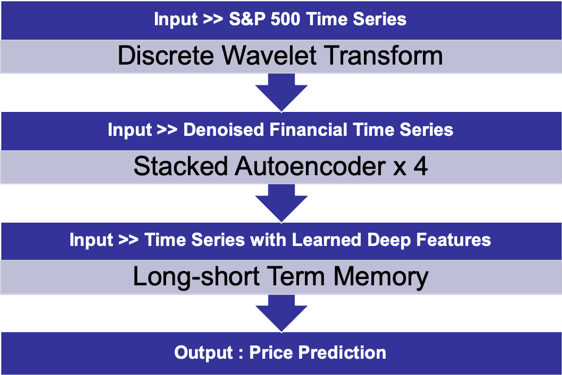
\includegraphics[width=0.6\linewidth]{./figs/flow}%\vspace{-0.4cm}
%\includegraphics[width=0.85\linewidth]{./FIGS/Overview_cropped}%\vspace{-0.2cm}
\caption{Overview of \scheme}
\label{fig-overview}
\end{center}
\vspace{-0.6cm}
\end{figure}

\subsubsection{Denoising using DWT (Wavelet Transform)}
First of all, we apply wavelet transform for data denoising. Wavelet transform has the ability to decompose complex information and patterns into elementary forms. It is applied for data denoising in this project because of its ability to handle non-stationary financial time series data, which is useful in handling highly irregular financial time series. We apply the Haar function as the wavelet basis function because it can not only decompose the financial time series into time and frequency domain but also reduce the processing time significantly. The wavelet transform with the Haar function as a basis has a time complexity of O(n) with n being the size of the time series. We first calculated wavelet coefficients for each data feature column, and designated a threshold to create the signals using thresheld coefficients. 

\subsubsection{Stacked Autoencoder}
After denoising, autoencoders are applied for layer-wise training for the OHLC variables and technical indicators. Single layer AE is a three-layer neural network, the first layer being the input layer and the third layer being the reconstruction layer, respectively. The second layer is the hidden layer, designed to generate the deep feature for this single layer AE. The aim of training the single layer AE is to minimize the error between the input vector and the reconstruction vector. The first step of the forward propagation of single layer AE is mapping the input vector to the hidden layer, while the second step is to reconstruct the input vector by mapping the hidden vector to the reconstruction layer. The activate function can have many alternatives such as sigmoid function, rectified linear unit (ReLU) and hyperbolic tangent. In this project, we set this to be a sigmoid function for all layers. The model learns a hidden feature from input by reconstructing it on the output layer. 

Stacked autoencoders is constructed by stacking a sequence of single-layer AEs layer by layer. The single-layer autoencoder maps the input daily variables into the first hidden vector. After training the first single-layer autoencoder, the hidden layer is reserved as the input layer of the second single-layer autoencoder. Therefore, the input layer of the subsequent AE is the hidden layer of the previous AE. 

For training, Adam optimizer is used for solving the optimization problem in SAEs, and completing parameter optimization. Each layer is trained using the same optimizer as a single-layer AE by and feeds the hidden vector into the subsequent AE. The weights and bias of the reconstruction layer after finishing training each single-layer AE are cast away. Depth plays an important role in SAE because it determines qualities like invariance and abstraction of the extracted feature. In this project, the depth of the SAE will be set to 4 with each layer having 10 hidden units.

\subsubsection{Long-short Term Memory}
After SAEs, we use the time series data as sequence to train the LSTM. LSTM networks consists of an input layer, several hidden layers and an output layer. The number of input layers is the same as the number of features. We choose LSTM because it doesn’t have the problem of vanishing gradients that a Recurrent Neural Network often has. The main drawback of RNN is that it cannot use previously seen data as the size of input sequences becomes larger. LSTM is a gated version of recurrent neural network that solves this problem. 

Another reason we use LSTM is because of the fact that in stock data pattern is the key factor to move the market in technical analysis. Hand-coded models such as clustering or feature extraction are sometimes difficult in time series data such as stock value. Therefore, the main purpose of the LSTM is to capture pattern throughout the time series data. For our LSTM model, the time step size is set to be 4, the batch size to be 60, and the hidden dimension to be 100. For training, we used the mean square error loss with Adam optimizer. 


\subsection{Applying NN with different stock features}
\label{sec-features}
\scheme\ uses different mathematical parameters as features. In stock price it is not enough to see only the price. There are several indicators that is used to predict different signals. \scheme\ uses those signal indicators as different features. However, features are more important for any machine learning model. If the features are good and it is learn-able then the model predictions are more accurate for financial data. Following sections describe the features first, then we describe how \scheme\ uses those in the NN model that we implemented in addition to \scheme\.

\subsubsection{Features}
There are several other feature maps that we use in our experiments are described below.
\begin{itemize}
    \item {\em Moving average convergence divergence (MACD):} MACD gives the convergence divergence of two period running exponential moving average (EMA). We use 12, 26 period EMA for calculating MACD. This features represents how price fluctuates over the period of time.
    
    \item {\em Relative strength index (RSI):} RSI is a momentum indicator that measures the magnitude of recent price changes to evaluate overbought or oversold conditions in the price of a stock or other asset. We choose this features to find out the market momentum at some particular point.
    
    \item {\em Bollinger Band (BB):} A Bollinger Band is a technical analysis tool defined by a set of lines plotted two standard deviations (positively and negatively) away from a simple moving average (SMA) of a stock price. It gives the range for a timeframe to fluctuate. This feature helps to get the highest and lowest point to fluctuate that helps to predict the director of the price.
    
    \item {\em Aroon Indicator:} Aroon is a statistical indicator that is used to identify the trend change in the stock.
    
    \item {\em Pivot points (PP): } PP gives several support and resistance level in price direction. Using this as a features helps to classify the direction of price trend.
    
\end{itemize}

\subsubsection{Model}

\begin{figure}[htpb]
\begin{center}
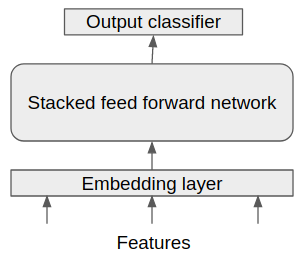
\includegraphics[width=0.35\textwidth]{./figs/stacked_NN}
\vspace{-0.2cm}
\caption{Stacked network with embedding layer for categorical bar prediction}
\label{fig_stackNN}
\end{center}
\vspace{-0.4cm}
\end{figure}


In this experiment we use different features as input and output is different bar predictions. All the bars are divided into several categories according to their body, head and tail (Figure~\ref{fig_stackNN}). At first we make a n-dimension embedding layer with all of our features together. Empirically we see that self learned embedding works better with this model. Embedding layer is passed through n-stacked feed forward network. The model outputs the prediction with softmax layer with cross-entropy loss. Dropout is used to make the training faster.

\subsubsection{A Glance on Implementation  }

Data preparation and handling are entirely conducted in Python 3.7 (Python Software Foundation, 2018), relying on the packages NumPy (Van Der Walt, Colbert, & Varoquaux, 2011), Pandas (McKinney, 2010). The neural network with LSTM are developed with keras (Chollet, 2016) on top of Google TensorFlow, a powerful library for large-scale machine learning on heterogenous systems (Abadi et al., 2015). The AutoEncoder and Wavelet Tranformation are processed by PyWavelets and PyTorch library respectively.